%  \documentclass{sig-alternate}
%\documentclass[conference]{IEEEtran}
\documentclass{sig-alternate-05-2015}


\usepackage{cite}
\usepackage{url}
\usepackage{color}
\usepackage{tikz}
\usepackage{balance}
\usepackage{caption}
\usepackage{soul} % Used for highlighting % \hl{this is some highlighted text}
\usepackage{cite}
\usepackage{xspace}
\newcommand{\etal}{{et al.\@\xspace}}

\usepackage[inline]{enumitem}
\setlist{leftmargin=1em}

%%%%
\usepackage{pgfplotstable}
\usepackage{pgfplots}
\pgfplotsset{compat=newest}

\usepgfplotslibrary{statistics}
\makeatletter

\pgfplotsset{
  /pgfplots/flexible yticklabels from table/.code n args={3}{%
    \pgfplotstableread[#3]{#1}\coordinate@table
    \pgfplotstablegetcolumn{#2}\of{\coordinate@table}\to\pgfplots@yticklabels
    \let\pgfplots@yticklabel=\pgfplots@user@ticklabel@list@y
  }
}

\pgfplotsset{
   boxplot/every median/.append style={thick},
   boxplot/every average/.append style={thick},
   boxplot/every outlier/.append style={thick}
}

\usetikzlibrary{patterns} %% Bar chart


\newcommand{\todo}[1]{\textcolor{cyan}{\textbf{[#1]}}}
\newcommand{\mei}[1]{\textcolor{green}{{\it [Mei: #1]}}}
\newcommand{\dan}[1]{\textcolor{blue}{{\it [Dan: #1]}}}
\newcommand{\yasmine}[1]{\textcolor{red}{{\it [Yasmine: #1]}}}
\newcommand{\pkm}[1]{\textcolor{magenta}{{\it [Pradeep: #1]}}}


\begin{document}

\title{XXXXX}
% Does Marshmallow help users remember the permissions?
% How Does Marshmallow affect
% Are Android's Run-Time Permission Requests Useful?
% Investigating the User's Perception and Comprehension of Android Run-Time Permissions: A Case Study

\author{
%
% 1st. author\
\alignauthor
XXXXXX 	\\
%	\affaddr{Software Engineering Department}\\
       \affaddr{Rochester Institute of Technology, Rochester, NY, USA}\\
       \email{\{xxxx,xxxxx,xxxxx\}@rit.edu}
       \alignauthor
} % Must not be a space above this


%   ynevse
%   pkmvse


\maketitle
\begin{abstract}


% Introduce the problem that we are trying to solve
% How did I do my study
% What did I find?

Android applications (apps) rely on a permission-based model to carry
out core functionality. The way that Android apps ask a user to accept
permissions has recently changed from being an all or nothing accept
or reject upon installation the application, to now asking for
permission at runtime. A primary goal of this change was to provide
users more control of the permissions their apps utilize. Do users
actually feel more comfortable with this change? Are they more
knowledgeable about the permissions their apps are using?

We conducted a large, in person study involving 322 participants from a diverse background
set to determine if this new permission model makes users feel more
comfortable and knowledgable about the permissions their apps are
using. We also sought to determine what impact providing a rationale
had on user's accepting permission requests.

We found that.....


%%% Update abstract with what our paper actually explored.



\end{abstract}

%%% Are these good keywords??? -- Check these
\begin{keywords}

Permission Comprehension, Android, Privacy

\end{keywords}


% Based on the venue, check to see what else needs to be added


\section{Introduction}
Android has become the world's most popular mobile platform, allowing
users to perform a variety of tasks that were previously unachievable
in a mobile environment. Android applications (apps) provide the user
with a diverse set of functionality allowing them to do everything
from posting their Facebook status, to performing banking
transactions. In order to perform various sensitive tasks, an app must
be granted appropriate permissions to carry out this functionality.
For example, if an app requests access to a user's contact list, the
app much explicitly ask the user for permission to access this
information. These app permissions serve as as an integral component
of the app's security by limiting access to this information and
functionality to other potentially malicious apps installed on the
user's device, but also in ensuring that a user is adequately able to
protect the information on their phone as they desire.


Modern smartphones and tablets are powerful devices as they possess ``computer-like'' computing capabilities, a collection of sensors, in addition to communication via WiFi, Bluetooth, and mobile phone networks. In order to protect the user's devices from potential security risks, an app must explicitly ask the user's permission to grant it access to some of the mobile device's sensitive resources. There are two main followed approaches in asking the users to grant permissions. The first approach is to  show the user all the permissions an app requests at installation time.  The other approach is to let the app requests permission while the user accesses different functionalities of the app. Previous research show that displaying all permissions requested by the app at installation time is non effective in informing the users about the potential risks of installing the app~\cite{Liu:2014:RMA:2566486.2568035, felt2011effectiveness}. This mechanism fails in communicating potential risks to the users. One reason behind this risk communication problem is labeling many permissions as ``dangerous permissions'' even when the app has a legitimate need for such permission(s)~\cite{sarma2012android}. When users install an app with ``dangerous permission'' and later find no negative consequences, they learn to ignore future warnings \cite{stewart1994intended, magat1988consumer}.  The second reason for the poor usability of this permission display approach is lack of adequate explanations, leaving the users confused with little understanding of what the permissions imply \cite{Felt:2012:APU:2335356.2335360, Kelley:2012:CPI:2426020.2426027}.


Since its inception, Android has used a system where users were asked to accept all of an app's permissions at install time. If they did not approve all of an app's requested permissions, they would not be allowed to install or use the app. This approach has been addressed in numerous works since its inception which have discussed privacy and security concerns with this model, and have proposed alterations to the model to enhance the user's experience in a variety of ways. For example, the previous model was criticized for not allowing users to selectively grant the permissions their apps were requesting and would force the user to either not use the app, or trust the app to not misuse their data or device, even for the permissions that they did not feel comfortable with.

Several works proposed solutions such as custom frameworks which would provide the user the ability to accept only a subset of the app's requested permissions~\cite{6949282, nauman2010apex, Conti:2010:CCP:1949317.1949355, Rasthofer:2014:DEC:2703000.2703303}. While such solutions would have provided the advantage of providing the user more control over their apps, the average Android user would be unlikely to conduct these somewhat complicated technical tasks. Additionally, these recommended changes would often require the user to root their phone, something which could lead to additional security threats~\cite{Rasthofer:2014:DEC:2703000.2703303}.


% With the increase in smart devices, apps, and malware, consumers should take precautions before installing apps.
%	With all the sensitive information on people's phones, the risks are very high


%%%%%% Include these as other papers to analyze
%
%
%Messing with Android?s Permission Model > 6296014
%
%X PeMo: Modifying Application?s Permissions and Preventing Information Stealing on Smartphones > 6949282
%
%
%
%Dr. Android and Mr. Hide: Fine-grained Permissions in Android Applications >
%	http://www.jeffvaughan.net/docs/drandroid-spsm12.pdf
%
%
%Curbing Android Permission Creep
%https://www.andrew.cmu.edu/user/nicolasc/publications/VCC-W2SP11.pdf
%
%
%Enhancing User Privacy on Android Mobile Devices via Permissions Removal
%
%
%Addroid: Privilege separation for applications and advertisers in android








%%% --> Go into greater detail about what some of these goals are

The manner in which apps requested permissions substantially changed
with the introduction of Android Marshmallow (Android M), which
adopted a process of an app asking for permissions at runtime instead
of install time. Users are now able to choose to provide an app
specific functionality while still installing and using an app
(without the functionality afforded by the permission), and even
change the app's permission settings whenever they pleased, even long
after installation.






%%% Probably add a few reasons for switching to M here
%The conversion to this new permission structure had several intentions including making users feel more comfortable, streamline the app installation process, and provide them more authority over their data and privacy, and allow for automatic updates since a user would no longer be required to accept all changed permissions at install time \cite{android_developer_URL}.


%%%%%




%% What do other works say we problems with the old model


Previous works have criticized the old model of requesting permissions at the beginning of the installation process in an all or nothing fashion for a variety of reasons including the inability of a user to alter permission settings based on situational constraints such as who is using the device or their location~\cite{Nauman:2010:AEA:1755688.1755732,Conti:2010:CCP:1949317.1949355}. According to Android, some of their primary goals for implementing the new permission model was to streamline the app installation and update process, while providing them more control over the permissions their apps used~\cite{android_developer_URL}. %%% Find other works which state this is bad from a permission comprehension perspective. This could be from non-Android related papers.



% M = streamline app install process, provide more control over permissions & functionality. Revoke permissions at any time
\pkm{Discuss these goals in greater detail. Also, identify other
concerns raised in the literature on the previous permissions model.
Doing this systematically will lead to research questions of
interest.}


We sought to determine if these goals were being met by performing a
large study involving 321 participants from  diverse backgrounds. Our
primary research questions were: \todo{add in RQs}

%\pkm{I am thinking whether to pose this as a pre-M vs. M study or more generically about permissions at install time vs. run time study. Are these two (install time and run time) the only two permissions models across platforms? If so, why not generalize the motivation for the study? If not, what are the other models? Can we generalize the experiment to test all major permission models?}

%% What are the current gaps


% Very clearly state the contributions of the paper


% The rest of the paper is organized as follows: In Section~\ref{sec:relatedworks}



%%% Primary Research questions

%   RQX: What effect does the new permission model have on a user's ability to recall an app's permissions?
%   RQX: What effect does the rationale have on a user's perception of a permission request?
%   RQX: Which model helps users feel more Comfortable?




\section{Background \& Related Work}
\label{sec:relatedworks}

%%% Add more to this depending on the conference we submit to

\subsection{Android Permissions}


Android apps operate under a privilege-separated system where each app
operates with a specific system identify, and each app is isolated
from all other apps on the device. More fine-grain functionally
enforces permissions on specific operations which the app may carry
out. For example, if an app wishes to access the internet, or the
user's contacts, the app will be required to be granted this
permission before the app has the ability to access this
functionality. Permissions are separated into several protection
levels, with the most important being \emph{normal} and
\emph{dangerous} permissions \cite{android_permissions_URL}.


%% DK: Removed 5'/30 - I didn't think it was useful
%%The dialog box shown by the system describes the permission group your app needs access to; it does not list the specific permission.  \todo{add this in someplace}



\begin{description}
  \item [Normal] permissions cover functionality that the app needs
    which are located outside of its sandbox, but are deemed to create
    very little risk to the user's privacy, or to other apps.  An app
    that requests a normal permissions is automatically granted this
    functionality. In Android Marshmallow, some normal permissions
    include \texttt{BLUETOOTH}, \texttt{ACCESS\_WIFI\_STATE} and
    \texttt{INTERNET}.

  \item [Dangerous] permissions are deemed to pose significant risks
    to the user's privacy, or to other apps installed on the device. One way that an app could pose a risk to another app is that through \emph{permission leaks}, which is when a less privileged app uses the granted permission of a more privileged app through the use of inter-process message components, or \emph{Intents}. Although the sharing of permission capabilities is an intended function of Android which serves as a way to make the user experience more friendly and not overwhelm them with permission requests~\cite{android_permissions_BestPractices_URL}, this can create security and privacy related issues in less secure or untrusted apps~\cite{FeltWMHC11}.

    The user must explicitly grant access to any dangerous permissions
    requested by the app.  In Android Marshmallow, some dangerous
    permissions include \texttt{READ\_CALENDAR}, \texttt{READ\_SMS}
    and \texttt{CAMERA}. In Android Marshmallow, all dangerous
    permissions belong to a specific permission group. For example,
    all dangerous permissions which are related to phone calls belong
    to the \emph{Phone} group. When an app requests a dangerous
    permission in a group which the user has already granted a
    permission in, the app automatically gains the ability to use that
    permission since the app has already been granted a permission in
    that group. For example, if the app requests the
    \texttt{CALL\_PHONE} permission, but the app has already been
    granted the \texttt{ADD\_VOICEMAIL} permission, the app will
    automatically gain access to the \texttt{CALL\_PHONE} permission
    since they both reside in the same group.
\end{description}

Prior to Android Marshmallow, the user was prompted to accept all
permissions, including the dangerous ones, when installing an app or
not install the app. The all or nothing ordeal was true when updating
an app, too. That is, a user had to accept all permissions and update
requires to install it or not install the update at all. Users were
also not able to change permissions after installation and the only
way to restrict an app's access to a specific permission was to
uninstall the entire app \cite{Wijesekera:2015:APR:2831143.2831175}.
In the past several years, there has been a substantial amount of
research recommending changes to the Android permission model ranging
from the creation of privacy profiles
\cite{Liu:2014:RMA:2566486.2568035} to more granular sets of Android
permissions \cite{7145666}. \pkm{If it is not too many
recommendations, let us list them all instead of just indicating the
range.}  %%% Much of this is a repeat from what I stated above. May want to think about reorganizing things
\dan{Is this redundant? Should we just move it?}


Marshmallow represented a significant change with how permissions were
handled in Android apps. Users would now be prompted about allowing an
app's permission requests at runtime, and not upon installing the
application. The intention is that this would make installing and
updating the app a simpler and an easier process while providing the
user greater access over the app, and therefore their privacy. The
user would also be able to use the app, but choose the permissions
they wanted to allow it to have, and even change their permission
decisions whenever they pleased. The developer would also have the
option of providing a \emph{rationale}, or further explanation, to the
user about why the app was asking for a particular permission.

%-- General info
%\cite{biswas2016android} %%% Probably not alll that useufl




\subsection{Related Work}


%   The first examining the M model
%   List all the papers which called for changes in the M structure
%   How were other user studies carried out (such as the felt study). Don'f forget to include some online or MTurk studies


%	What have been other proposed models
%	What works have found issues with the current model
%	What other studies have been done on permission and users (For both Android and not Android)
%	


%   Enhancement on privacy permission management for Android apps



% 	A conundrum of permissions: Installing applications on an Android smartphone > http://infosecon.net/usec12/papers/kelley-usec12.pdf
% 	Short Paper: Enhancing Users? Comprehension of Android Permissions


%	Investigating Users? Reaction to Fine-Grained Data Requests: A Market Experiment > http://www.bodden.de/pubs/erk+15investigating.pdf   --> Good related works section


%% When It?s Better to Ask Forgiveness than Get Permission: Attribution Mechanisms for Smartphone Resources >> Good overview of related works and when to ask for permissions

% Felt:2012:APU:2335356.2335360

%
%   A  Conundrum of Permissions: Installing Applications on an Android Smartphone
%   Claim What You Need: A Text-Mining Approach on Android Permission Request Authorization


% Android Permissions: User Attention, Comprehension, and Behavior
% "This would give users finer-grained control over the resources that applications have access to. We do not recommend adopting this proposal until user understanding of permissions can be improved with other measures. The low comprehension rates suggest that users cannot currently make informed decisions about individual permissions"
%	Maybe put this into the discussion


%% Lots of research on update messages and wording
%	How does this message make you feel? A study of user perspectives on software update/warning message design

% Mobile App Installation: the Role of Precautions and Desensitization
%	Through a survey of 209 participants, a prediction model was created that attempts to predict whether respondents would download applications asking for excessive permissions. The model results indicate those that take more precautions are less likely to download apps requesting excessive permissions.


% Mobile App Installation: the Role of Precautions and Desensitization - Seems to have been a very different kind of study, but with some overlapping RQs
%	Talks about some app permission tendencies
%	Good paper that talks about 6.0 a bunch
%	Good source of other papers for our lit review
%	Interesting: "A higher percentage of females will resist installing apps with excessive permission requests than males."



%   Look at the references in "Follow My Recommendations: A Personalized Privacy Assistant for Mobile App Permissions"


\section{Methodology} % User Study
\label{sec: method}


In the following section, we will discuss our hypothesis before conducting the study, our study design, and how our study was conducted.

\subsection{Terms}
Several terms that will be used in our study include:

\begin{itemize}
	\setlength{\itemsep}{.8pt}
    	\setlength{\parskip}{0pt}
    	\setlength{\parsep}{0pt}
	\item \textbf{Pre-M}:  Android API $\leq 22$, which used the old Android permission model of asking users to accept or reject all requested permissions at install time.
	\item \textbf{Marshmallow}:  Android API $\geq 23$ which allows apps to ask users to accept or reject permissions runtime.
	\item \textbf{M--Rationale}:  The app running on Android Marshmallow, and where permission requests are given a short rationale as to why they are needed before prompting the user to accept or reject the permission at runtime.
	\item \textbf{M--No rationale}:  The app running on Android Marshmallow, but where no extra explanation of why the permission is required is provided to the user.


\end{itemize}

%\pkm{Include terminology here, e.g., Pre-M: Pre marshmallow permissions model, M--No rationale: Marshmallow permissions model without including a rationale for a permission.  You can then use these terms in the hypotheses.}

% Mention the number of users and then talk about things like how many users were removed for being under 18
%


\subsection{Hypothesis}

\todo{work on telling a story with these}\todo{Add in hypothesis from MTurk study}
%% Use "Mobile App Installation: the Role of Precautions and Desensitization" as a guide
%	FInd other papers we can cite here

In order to guide our research, we developed several hypothesis:



\begin{enumerate}

	\item The new permission model affords users greater control to choose the permissions that their app uses, granting some permissions an apps requests, but not others. Users may also decide to alter an app's granted permissions at any time after the installation process. A primary goal of the new permission model was to give users more control over the app's permissions ~\cite{android_developer_URL}.


Granting permissions to an app is accompanied by risks such as downloading malicious software, and leakage of personal information. An important factor that affects risk assessment is the amount of control that users believe they have over the risky activity. Users perceive controllable activities (e.g. toggle permissions) as less risky than uncontrollable activities \cite{hale1987individual}.

$H_0$ = Marshmallow will not impact on how secure a user feels when using the app.

$H_1$ = Marshmallow will make users feel more secure with using the apps.


%% Cite paper that showed that this was a problem


\item Marshmallow adds the ability for developers to provide a greater context as to why the app is requesting its permissions. For example, developers may choose to make use of such functionality as~\emph{shouldShowRequestPermissionRationale()} to provide more information in a pop-up about why an app is requesting a permission. The role of information is vital in supporting decision making. According to the information processing theory, when people are provided with useful information, they are enabled to engage in analytical and rational thinking \cite{epstein1994integration}. In the context of technological risks, users can assess the tradeoff between risk level and perceived benefit when proper information are conveyed to them \cite{fischhoff1978safe}. Such information could be scenario information or frequency information \cite{slovic2005affect}.\dan{clean up this wording}



Two methods of measuring how helpful these rationales are for users is how well they help a user to understand the permission being requested, and if it has any impact on their ability to recall the permissions the app has asked for. %% Not sure that recall will be very useful

$H_0$ = The rationale functionality that Marshmallow provides will not help a user to better understand the permissions that the app is requesting.

$H_1$ = The rationale functionality in Marshmallow will make it easier for a user to understand the permissions an app is requesting.


$H_0$ = The rationale provided in Marshmallow will not help users to recall the permissions the app asked for.

$H_1$ = The rationale provided in Marshmallow ill impact the user's ability to recall the permissions the app asked for.




\item A basic premise behind the Android permission structure is that it is intended to inform users about the risks of installing applications ~\cite{android_security_overview_URL}. Previous research has shown that users do not typically read or comprehend the permissions that their app has requested very well~\cite{Felt:2012:APU:2335356.2335360, Kelley:2012:CPI:2426020.2426027}. Users can only make correct security decisions for their device if they correctly understand what the permissions mean. A system which is better able to inform users about the permissions the app was requesting would allow them to make more comfortable, appropriate choices about their privacy when using the app on their device. %%% Find something to back this up?

$H_0$ = Marshmallow will have no impact on a user's ability to correctly recall the permissions an app has asked for.

$H_1$ = Marshmallow will have a statistically significant impact on a use's ability to recall the permissions their app has asked for


\item Previous research has shown that most users do not pay attention to the permissions being request by their apps


~\cite{Felt:2012:APU:2335356.2335360}

\todo{cite}\todo{finish.....} % What does the other research say? Why is this important?





$H_0$ = The new permission model of asking users to accept permissions at runtime does not impact how much a user pays attention to the permissions being requested by their app.

$H_1$ = Asking users to accept or reject permissions at runtime will allow users to


\dan{I am not sure how to measure this... leave it in??}



%\item XXXX
%
%Ho = XXXX
%
%H1 = XXX



\end{enumerate}


% Background
% H1









% 	http://www.pacis-net.org/file/2015/3002.pdf


%	****


%
%\pkm{Hypotheses always come in pairs: null and alternate. The ones
%  below all seem alternates. It is a good practice to include a null
%for each.}
%\begin{enumerate}
%
%%%% Provide more citations and reasons why we believe this
%
%	\item \textbf{Marshmallow helps users feel more secure using the apps}:  The new permission model affords users greater control to choose the permissions that their app uses. We believe that this will make users feel more secure with using the apps. Our
%
%
%	\item \textbf{ Permissions in Android M are easier to understand and recall if we add meaningful rationale to the requested permissions}:  (find external works to back this up or support it) - \todo{Find reasons to back up the way I believe that I do}
%    \pkm{Understand and recall should be two different hypotheses}
%	\item \textbf{Most users still have poor comprehension of Android permissions}:  Previous research has also shown that the majority of users do not properly comprehend what permissions actually mean ~\cite{Felt:2012:APU:2335356.2335360}. We believe that our findings for both the Pre-M and Marshmallow versions of the app will support these previous findings. \todo{add more citations}
%    \pkm{Not a concrete hypothesis. How many users is most? How will
%      you validate such a hypothesis? Instead,
%      considering the overall objective of the paper, pose the
%      hypothesis as something like M users comprehend permissions
%      better than Pre-M users. I would imagine this to be true since M
%      asks for permissions ``in-context.'' If the corresponding null
%      hypothesis cannot be rejected, then it is a point for
%    discussion.}
%	\item \textbf{Providing a rationale will help users feel more comfortable with accepting permissions}:  XXXXX\todo{find rationale}
%    \pkm{I read the Android developer guide's take on rationale. It
%    recommends using rationale when the need for a permission is not
%  obvious. So, I am wondering whether rationale always helps or not,
%e.g., for a camera app, does including a rationale for the camera
%permission help?}
%	\item \textbf{Most users will continue to pay little attention to permissions}:  Previous research conducted on the Pre-M permission model has shown that most users do not pay attention to permissions when installing an app~\cite{Felt:2012:APU:2335356.2335360}. Although the new Marshmallow model will provide users with more control, and in many ways make them more aware of the permissions they are installing, we still believe that permission attention will continue to be a problem.
%    \pkm{Again, not a concrete hypothesis.}
%%	\item \textbf{Danz}:
%%	\item \textbf{Danz}:
%%	\item \textbf{Danz}:
%
%\end{enumerate}
%



%%% Make sure to find other works to back up my hypothesis





\section{Study Design}
\label{sec:studyDesign}

In the following sections, we will describe how we conducted both our in person, and online study using MTurk.

\subsection{In Person Study} % Find a better name for this
%% Mention the primary components of our study
Our study was comprised of three primary components: User Recruitment, the Tic-tac-toe app, and Questionnaire, which we will describe.

\subsubsection{Recruitment}

Our human study was conducted at Imagine RIT\footnote{\url{http://www.rit.edu/imagine/}}, a single day event where thousands of members of the community visit the RIT campus and view a variety of scientific and educational venues ranging from robotics, software projects, and engineering activities. With the assistance of student volunteers, we set up two tables with six MacBook laptops running an Android emulator. Two laptops were running the emulator with API 22 (Pre-M), while the other four were running API 23 (Marshmallow). Participants were recruited by asking visitors passing by our table if they would like to participate in an Android study. Users were only provided vague details about the study being about Android permissions in the event pamphlet.

\subsubsection{Application}

We developed a simple Tic-tac-toe app for use in our study, which
contained the following permissions: \texttt{ACCESS\_FINE\_LOCATION},
\texttt{GET\_ACCOUNTS} and \texttt{READ\_PHONE\_STATE}. We selected
these permissions since they have been identified as commonly used
permissions in Ad libraries~\cite{liu2015efficient}. \dan{describe these permissions more?}  When beginning
to use the app, users were told to act like they were using the app on
their personal device and were randomly asked to participant using one
of three nearly identical versions of the app:

\begin{enumerate}

    \item  \textbf{Android Pre-Marshmallow} (API 22): Users were asked to accept or deny all app permissions at install time, a process which replicates how Android has asked users for permissions since its inception.

    \item  \textbf{Android Marshmallow - No Rationale} (API 23) Users were asked to accept or reject permissions at runtime. At the beginning of the game, participants were told that the app needed to locate people around them and the user was asked if they wanted to allow the app to access the device's location. After playing the game, the app asked for the permissions to make calls and access the user's contacts.

    \item  \textbf{Android Marshmallow - With Rationale} (API 23): This version of the app was identical to the No Rationale version, except that a rationale was provided to the user before being prompted for their permission. For example, before asking for permission to access the user's contacts, a rationale stated that ``This App needs to access your contacts to share results.''

\end{enumerate}

Both Marshmallow versions of the app were connected to a database which recorded whenever a user accepted or denied a permission. Since all permission requests are made at installation for Pre-M apps, there was no data to record for this API level.

The app began by asking users to start a new game, and was followed by participants selecting several area participants to play against. Since the primary objective of the research was to understand how users react to the new permission model, we felt comfortable mocking out this functionality in the app. The participants would then play the game and were notified of their victory or defeat at the conclusion of the game. Once the game was completed, users were asked to share their results with the contacts on their device.

\subsubsection{Questionnaire \& Exit Survey}

Before using the app, participants were initially asked to provide basic information about themselves such as age, gender, highest level of education, and how long they have used Android. Participants were not required to have ever used Android. After playing the game, participants were then asked to fill out the second portion of the questionnaire, which was nearly identical for all three of the user groups, except for certain questions pertaining to each group such as how helpful the permission rationale was, or if the user felt comfortable with accepting or rejecting permissions at runtime. Users were not allowed to go back and use the game to assist them in answering any of the questions, and were told to do the best they could in accurately answering all questions.




\subsection{Online Study Using MTurk}






Although we collected results from over \todo{XXX} participants from a diverse set of backgrounds and age ranges, we still felt that there were some areas of our study to improve upon. For example, we wanted to include a second application into our study to see how our results were affected when the users were using more than one application in the analysis. We also wanted to include more variability in the rationale including alternating providing permission rationales to see any affect that would have on the user's responses. Due to the nature of our audience, we were limited in the amount of study time we had with the participants in our in-person study. In order to expand upon our results from our in person study, we decided to conduct a larger online study using Amazon Mechanical Turk (MTurk)\footnote{\url{https://www.mturk.com}}, which is an online crowdsourcing environment which we used to recruit participants for our online study.


% Show that it has been used in other studies???


%   What holes were we trying to fill
%   More users trying multiple apps (this was difficult to accomplish with the limited time most users were willing to spend on the in person study)
%


%   Add another app into the equation. -> Time before answer questions, confusion with other apps to create a more realistic scenario -> Couldn't do in person due to time constraints
%   Create more variability with the rationale messages
%       % Quality of messages, show messages sometimes, but not others



\subsubsection{Recruitment}


%   	What locations did they come from
%   	How much were they paid
%   	Did we advertise it at all
%   	Look @ how other papers describe their MTurk recruiting process.
%	How many users for each portion of the study
%	Talk about the demographics of our participants. Who did we ultimately get?
%	How long did it take each user to complete the activity - Briefly mention this
%	From start to finish, how long was the study up on MTurk for
%	Decent paper to use as template for describing MTurk "Effective Risk Communication for Android Apps"




\subsubsection{Applications}

We used two apps for our MTurk online study, a Tic-tac-toe game similar to the one used in our in person study, and a `Restaurant Evaluation' app. These apps were hosted on an online emulator, Appetize.io\footnote{\url{https://appetize.io}} which allowed study partipants to use the apps in an online environment through their web browser. We chose to use an online emulator for our study to make it was easy as possible for participants to use our apps, and to eliminate variability and mistakes that could arise from participants installing the apps on their own devices. We chose https://appetize.io because

Unfortunately, the emulator did not allow

API version used


%   How were they constructed
%   Pre-M apps emulated the permission request screen
%	Talk about the four different versions of the apps
%   Talk about the variability in the rationales of the apps. GG, GB, BG, BB


%   Make sure to update any information on these






\noindent
\textbf{Tic-tac-toe: }The primary differences between the Tic-tac-toe game used in this MTurk study, and


%   Why we chose these apps
%   How many permissions did they each request


\noindent
\textbf{Restaurant: }XXX


%   Why we chose these apps
%   How many permissions did they each request




\subsubsection{User Survey}



\section{Results}



Our work was driven by XXX primary research questions:\\

\textbf{RQX: What effect does the new permission model have on a user's ability to recall an app's permissions?}


A primary goal of the new permission model was for users to be more knowledgable about the permissions their apps were using~\cite{android_developer_URL}. It is important for a user to recall \todo{Yasmine: Finish}



As part of our user study, we asked users how easy it was to recall the permissions they accepted and rejected

%\todo{Yasmine: Find citations about why it is important for users to know the permissions in their app}

%%


% Give more of an introduction as to what we did

%A primary goal of the new permission model was for users to be more knowledgable about the permissions their apps were using.


 %% Pradeep: Let's provide the statistics for the following questions and show them in the way that you feel is the most appropriate:

%	How easy was it to recall what permissions you accepted?
%	How easy was it to recall what permissions you rejected?

\begin{figure}[!htb]
  \centering
  \begin{tikzpicture}
    %\tikzstyle{every node}=[font=\small]
    \begin{axis}[
	y=0.6cm,
	ytick={1,2,3},
	yticklabel style={align=center},
	yticklabels={Pre-M,M--No rationale,M--Rationale},
	width=6cm,
	xtick={1,2,3,4,5,6,7},
	xlabel={Ease of remembering permissions accepted},
	xlabel style={align=center},
	boxplot/average=auto,
	%title style={align=center},
	%title={Permissions accepted},
	%title style={yshift=-1ex,},
        %cycle list name=colorbrewer-RYB3,
	]
	\addplot+[boxplot]
	table[x expr=\coordindex, y index=0, col sep=comma]
	{ease-recall.csv};

	\addplot+[boxplot]
	table[x expr=\coordindex, y index=1, col sep=comma]
	{ease-recall.csv};

	\addplot+[boxplot]
	table[x expr=\coordindex, y index=2, col sep=comma]
	{ease-recall.csv};
    \end{axis}
  \end{tikzpicture}

  \vspace{1em}
  \begin{tikzpicture}
    %\tikzstyle{every node}=[font=\small]
    \begin{axis}[
	y=0.6cm,
	ytick={1,2,3},
	yticklabel style={align=center},
	yticklabels={Pre-M,M--No rationale,M--Rationale},
	%ytick=\empty,
	width=6cm,
	xtick={1,2,3,4,5,6,7},
	xlabel={Ease of remembering permissions rejected},
	xlabel style={align=center},
	boxplot/average=auto,
	%title style={align=center},
	%title={Permissions rejected},
	%title style={yshift=-1ex,},
        %cycle list name=colorbrewer-RYB3,
	]
	\addplot+[mark=x,boxplot]
	table[x expr=\coordindex, y index=3, col sep=comma]
	{ease-recall.csv};

	\addplot+[mark=x,boxplot]
	table[x expr=\coordindex, y index=4, col sep=comma]
	{ease-recall.csv};

	\addplot+[mark=x,boxplot]
	table[x expr=\coordindex, y index=5, col sep=comma]
	{ease-recall.csv};
    \end{axis}
  \end{tikzpicture}
  %\vspace{-2ex}
  \caption{Ease with which participants remember the permissions they
  accepted and rejected.}
  \label{fig:personality-strategy-novelty}
\end{figure}


We next sought to determine if users were actually able to recall the
permissions the app requested. As part of our post activity survey, we
asked to users to select all the permissions the app used from a list
of six possible options. We then measured the precision, recall and
F-score of the user's ability to correctly recall the permissions the
app had used. The results of this analysis are shown in
Figure~\ref{fig:remember}.


\begin{figure}[!htb]
\centering
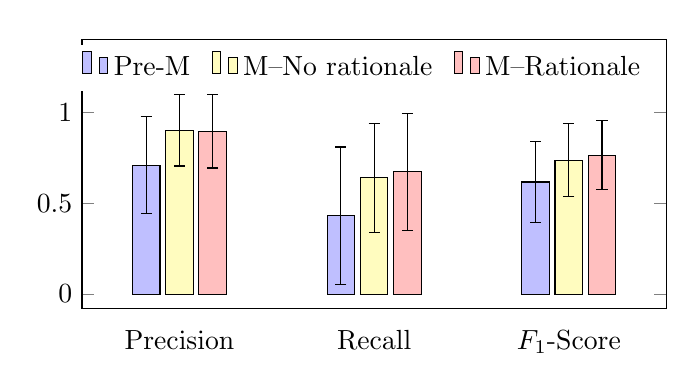
\begin{tikzpicture}
\begin{axis}[ybar,
    width=9cm,
    height=5cm,
    xtick={1,2,3},
    xticklabels={Precision, Recall, $F_1$-Score},
		enlarge x limits=0.25,
		xtick style={draw=none},
		ymax=1.4,
		legend style={draw=none,legend columns=-1,
		  /tikz/every even column/.append style={column sep=0.2cm}},
    ]

\addplot[
    fill=blue!25,
    draw=black,
    point meta=y,
    error bars/.cd,
        y dir=both,
        y explicit
]
table [y error=error] {
x y error
1 0.7091 0.2652
2 0.4316 0.3772
3 0.6164 0.2211
};

\addplot[
    fill=yellow!25,
    draw=black,
    point meta=y,
    error bars/.cd,
        y dir=both,
        y explicit
]
table [y error=error] {
x y error
1 0.9009 0.1967
2 0.6394 0.3
3 0.7360 0.2013
};

\addplot[
    fill=red!25,
    draw=black,
    point meta=y,
    error bars/.cd,
        y dir=both,
        y explicit
]
table [y error=error] {
x y error
1 0.8958 0.2026
2 0.6731 0.3217
3 0.7636 0.1904
};
\legend{Pre-M,M--No rationale,M--Rationale};
\end{axis}
\end{tikzpicture}
\caption{Participants' ability to remember permissions.}
\label{fig:remember}
\end{figure}


There was only a very small difference in the results between the `M - With Rationale' and `M - Without Rationale' groups, which is not surprising since the same permission requests were still shown at the same time to the users, with only an extra reasoning dialog shown to the with rationale group. However, there was a large difference in the three evaluated groups between the two `M' groups, and the `Pre-M' group. This demonstrates that users were able to more accurately able to recall the proper requested permissions for each of the Marshmallow groups in comparison to the Pre-M group. With the Pre-M model, users are shown the app's permissions at install time. Very frequently, users would quickly skim through this list in an attempt to use the app as soon as possible. Users also voiced their displeasure with the permission model in their feedback, with one user stating: ``Either you accept the condition of permission or you cannot install the application. that's a really annoying thing. I'd like to know why a particular app needs the permissions it needs.'' This lack of attention to the permissions in the Pre-M model is supported by previous research which demonstrates that few users pay attention to permissions when installing an app and that very few users are able to correctly recall the permissions an app uses~\cite{Felt:2012:APU:2335356.2335360}.




This demonstrates that % State the importance of these results







\todo{See if there is a correlation between the ability to recall permissions and if users said it was easy - Do on an individual level}


\textbf{Discussion:}
% Talk about ramifications/implications here. What is the "so what" ?

%	The new model does help users understand permissions better
%	Developers may want to switch to supporting the new model
%	Encourage end users to swtich (maybe talk about the fragmentation of Android and how updating is hard)
%	How many users knew the version of Android they were running




\textbf{RQX:} What effect does the rationale have on a user's perception of a permission request?

%% Also talk about the quality of the rationale in here


We next sought to determine the effect that providing a meaningful rationale had on a user accepting or denying a permission request. In order to explore this question, we provided users with nearly two identical versions of the same app, with the only difference being that one version provided users with a meaningful rationale as to why the permission was required. Whenever a user accepted or rejected a permission request, we recorded these results in a remote database. In the `With Rationale' version of the app, we provided a meaningful rationale as to why the app was requesting the permission before asking the user for their location (\texttt{ACCESS\_FINE\_LOCATION}) and if the app could have access to the contacts information on the device (\texttt{GET\_ACCOUNTS}). In order to act as a control between the two groups, we provided no rationale for the \texttt{READ\_PHONE\_STATE} permission. \dan{best way to say this?} The results of this analysis are shown in Table~\ref{table:permAcceptance}.

%Using the~\emph{shouldShowRequestPermissionRationale()} function, each user

\begin{table}[h]
\begin{center}
\caption{Permission Model User Acceptance} %%% Change the title
\label{table:permAcceptance}
\begin{tabular}{l|l|l}

{} &\multicolumn{2}{ c }{\bfseries Acceptance Rate} \\ \hline
    \bfseries Permission Group & \bfseries Rationale  & \bfseries No Rationale  \\ \hline\hline
%    \bfseries ACCESS\_FINE\_LOCATION & 0.95	 &	0.86  \\ \hline
%    \bfseries GET\_ACCOUNTS & 0.62 &	0.49  \\ \hline
%    \bfseries READ\_PHONE\_STATE & 0.59  &	0.57  \\ %\hline    			
    \bfseries Location & 0.95	 &	0.86  \\ \hline
    \bfseries Contacts & 0.62 &	0.49  \\ \hline
    \bfseries Phone & 0.59  &	0.57  \\ %\hline    			




\end{tabular}

\end{center}

\end{table}


%%% Does this rationale help users to feel more comfortable?

 These results demonstrate how a meaningful rationale can influence a person to accept



 Although we have found meaningful results, we believe that there is substantial room for future research in this area. For example, \todo{talk about the future work}


%% Discuss these results a bit


%% Demonstrates the need for future work in this area

 %  How the rationale






%%%% What is the takeaway messsage for developer's



\textbf{Discussion:}
% Talk about ramifications here.  What implications arise from this

%	Developers should use rationale
%	




\textbf{RQX:} Which model helps users feel more Comfortable?










%%% Further explore some of the statistics here

%      How many got the other permission questions correct
%      What do the general survey results say





%%%% So What

%   Developers should switch over to the new model
%   Demonstrates that the new model is effective
%




\section{Other Observations}
\label{sec:miss}


%   	How many users could correctly answer questions about location, phone calls, accounts
%		Link into other works which say that users don't know much about privs
%   	Do demographics/time of Android use play a role in things?
%   	What were some general user preferences about how they felt?
%	Difference in how users thought they understood permissions, compared with how well they actually did.


\section{Limitations \& Future Work}
\label{sec:futurework}

%% Did not have users use Marshmallow for extended periods of time, meaning that they did not use many of the other features such as altering permissions after installation or viewing all the apps that use a particular permission in the app menu

% Performed study only on laptop. Did not use actual Android device
% Do a longer, lab study like was done with Felt

%   What do other papers that do in person & MTurk studies say about limitations. Borrow from some of their identified limitations.

% Limitation: We do not study if users change their mind after 1st installing the app


\section{Conclusion}
\label{sec: conclusion}



\section*{Acknowledgment}

We would like to thank the following students for their contributions to the project: Hussein Talib, Cesar Fernandez, Silva Matti, Paula Garcia, Chris Lentner, Daniel Santoro, Taylor Corrello, Jodie Miu, George Hearde, and Kocsen Chung. This work was partially funded through a development grant from the Rochester Institute of Technology.



\balance % enable this
\bibliographystyle{abbrv}
\bibliography{MPermissions}

% That's all folks!
\end{document}


% ************************

%%%%% Notes
%   Make sure that it is: Tic-tac-toe


%% Primary Research Questions
%	Do users recall M permissions more?
%	Does rationale help users feel more comfortable?
%	Do Android users actually understand permissions better than non-users?
%	


%%% Todo
%




%%% Venues



%%% Future work
%   Have rationales hide totally unnecessary permissions which could create privacy concerns
%   How can the rationale be worded to have users accept it?
%   Crowdsource the rationale



%%%%% Usability study info



 

